%%%GKA_PR_template.tex

\documentclass[a4paper]{article}
\usepackage{praktikum}
\begin{document}
	
%%
%% Bitte das Deckblatt nicht verändern


\thispagestyle{empty}
\begin{center}

    {\large {\bf   BAI3-GKA WiSe2§ \\ Graphentheoretische Konzepte und Algorithmen \\[5mm]} }
    
{\huge Praktikumsaufgabe-Template  \\[5mm] Deckblatt}\\

\end{center}
Geben Sie bitte Ihre Namen, Ihr Team und die Gruppe  an:\\ 
				\begin{tabular}[t]{|r|l|}
				 \hline
%%%%				
%%%% Bitte  Ihren Namen und  Ihr Team und die Gruppe angeben
				GKA-Gruppe&                 \raisebox{-3mm}{\rule[8mm]{100mm}{0mm} }\\ \hline    
				Team &                                                        \\ \hline			
				& \textit{ Fabian Gottong }               \\ \hline    
				& \textit{ Anton Bosenick }               \\ \hline			
				& \textit{ Jonas Metzger }             \\ \hline  			
				\multicolumn{2}{c}{}\\  			
				\multicolumn{2}{l}{Bearbeitete Themen in Stichpunkten:}\\			
				\multicolumn{2}{c}{}\\  \hline
				Name &                \\ \hline    
				Name&                  \\ \hline			
				Name&                \\ \hline 		
				\multicolumn{2}{c}{}\\  			
				\multicolumn{2}{l}{Geschätzte Arbeitszeiten in Stunden:}\\			
				\multicolumn{2}{c}{}\\  \hline
				Name&                 \\ \hline    
				Name&                  \\ \hline			
				Name&                \\ \hline 			
				\end{tabular}
~\\[4mm]
		
		
\vfill


\newpage
\section{Dokumentation Ihrer Implementierung}

Hier Ihre Doku .....
\\ ... und vergessen Sie Ihre Quellen nicht, z.B. \cite{KN2012} und Ihre Abbildungen nicht, z.B. Abb.~\ref{fig:bild}.
  


\section{Beantwortung der  Fragen}
\begin{enumerate}
						\item Antwort auf die erste Frage
						\item 
					\end{enumerate}


\section*{Abbildungen}


\begin{figure}[h]
	\centering
		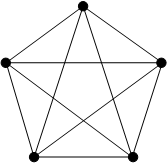
\includegraphics[width=0.50\textwidth]{Figs/Bild.png}		
	\caption{Beispiel für eine Abbildung}
	\label{fig:bild}
\end{figure}



\bibliographystyle{alpha}
\bibliography{mybib}
%%%%GKA_PR_template.tex

\documentclass[a4paper]{article}
\usepackage{praktikum}
\begin{document}
	
%%
%% Bitte das Deckblatt nicht verändern


\thispagestyle{empty}
\begin{center}

    {\large {\bf   BAI3-GKA WiSe2§ \\ Graphentheoretische Konzepte und Algorithmen \\[5mm]} }
    
{\huge Praktikumsaufgabe-Template  \\[5mm] Deckblatt}\\

\end{center}
Geben Sie bitte Ihre Namen, Ihr Team und die Gruppe  an:\\ 
				\begin{tabular}[t]{|r|l|}
				 \hline
%%%%				
%%%% Bitte  Ihren Namen und  Ihr Team und die Gruppe angeben
				GKA-Gruppe&                 \raisebox{-3mm}{\rule[8mm]{100mm}{0mm} }\\ \hline    
				Team &                                                        \\ \hline			
				& \textit{ Fabian Gottong }               \\ \hline    
				& \textit{ Anton Bosenick }               \\ \hline			
				& \textit{ Jonas Metzger }             \\ \hline  			
				\multicolumn{2}{c}{}\\  			
				\multicolumn{2}{l}{Bearbeitete Themen in Stichpunkten:}\\			
				\multicolumn{2}{c}{}\\  \hline
				Name &                \\ \hline    
				Name&                  \\ \hline			
				Name&                \\ \hline 		
				\multicolumn{2}{c}{}\\  			
				\multicolumn{2}{l}{Geschätzte Arbeitszeiten in Stunden:}\\			
				\multicolumn{2}{c}{}\\  \hline
				Name&                 \\ \hline    
				Name&                  \\ \hline			
				Name&                \\ \hline 			
				\end{tabular}
~\\[4mm]
		
		
\vfill


\newpage
\section{Dokumentation Ihrer Implementierung}

Hier Ihre Doku .....
\\ ... und vergessen Sie Ihre Quellen nicht, z.B. \cite{KN2012} und Ihre Abbildungen nicht, z.B. Abb.~\ref{fig:bild}.
  


\section{Beantwortung der  Fragen}
\begin{enumerate}
						\item Antwort auf die erste Frage
						\item 
					\end{enumerate}


\section*{Abbildungen}


\begin{figure}[h]
	\centering
		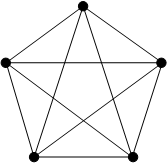
\includegraphics[width=0.50\textwidth]{Figs/Bild.png}		
	\caption{Beispiel für eine Abbildung}
	\label{fig:bild}
\end{figure}



\bibliographystyle{alpha}
\bibliography{mybib}
%%%%GKA_PR_template.tex

\documentclass[a4paper]{article}
\usepackage{praktikum}
\begin{document}
	
%%
%% Bitte das Deckblatt nicht verändern


\thispagestyle{empty}
\begin{center}

    {\large {\bf   BAI3-GKA WiSe2§ \\ Graphentheoretische Konzepte und Algorithmen \\[5mm]} }
    
{\huge Praktikumsaufgabe-Template  \\[5mm] Deckblatt}\\

\end{center}
Geben Sie bitte Ihre Namen, Ihr Team und die Gruppe  an:\\ 
				\begin{tabular}[t]{|r|l|}
				 \hline
%%%%				
%%%% Bitte  Ihren Namen und  Ihr Team und die Gruppe angeben
				GKA-Gruppe&                 \raisebox{-3mm}{\rule[8mm]{100mm}{0mm} }\\ \hline    
				Team &                                                        \\ \hline			
				& \textit{ Fabian Gottong }               \\ \hline    
				& \textit{ Anton Bosenick }               \\ \hline			
				& \textit{ Jonas Metzger }             \\ \hline  			
				\multicolumn{2}{c}{}\\  			
				\multicolumn{2}{l}{Bearbeitete Themen in Stichpunkten:}\\			
				\multicolumn{2}{c}{}\\  \hline
				Name &                \\ \hline    
				Name&                  \\ \hline			
				Name&                \\ \hline 		
				\multicolumn{2}{c}{}\\  			
				\multicolumn{2}{l}{Geschätzte Arbeitszeiten in Stunden:}\\			
				\multicolumn{2}{c}{}\\  \hline
				Name&                 \\ \hline    
				Name&                  \\ \hline			
				Name&                \\ \hline 			
				\end{tabular}
~\\[4mm]
		
		
\vfill


\newpage
\section{Dokumentation Ihrer Implementierung}

Hier Ihre Doku .....
\\ ... und vergessen Sie Ihre Quellen nicht, z.B. \cite{KN2012} und Ihre Abbildungen nicht, z.B. Abb.~\ref{fig:bild}.
  


\section{Beantwortung der  Fragen}
\begin{enumerate}
						\item Antwort auf die erste Frage
						\item 
					\end{enumerate}


\section*{Abbildungen}


\begin{figure}[h]
	\centering
		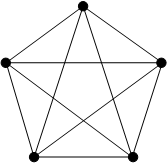
\includegraphics[width=0.50\textwidth]{Figs/Bild.png}		
	\caption{Beispiel für eine Abbildung}
	\label{fig:bild}
\end{figure}



\bibliographystyle{alpha}
\bibliography{mybib}
%%%%GKA_PR_template.tex

\documentclass[a4paper]{article}
\usepackage{praktikum}
\begin{document}
	
\input{deckblatt}
\newpage
\section{Dokumentation Ihrer Implementierung}

Hier Ihre Doku .....
\\ ... und vergessen Sie Ihre Quellen nicht, z.B. \cite{KN2012} und Ihre Abbildungen nicht, z.B. Abb.~\ref{fig:bild}.
  


\section{Beantwortung der  Fragen}
\begin{enumerate}
						\item Antwort auf die erste Frage
						\item 
					\end{enumerate}


\section*{Abbildungen}


\begin{figure}[h]
	\centering
		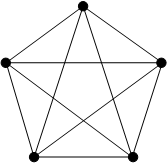
\includegraphics[width=0.50\textwidth]{Figs/Bild.png}		
	\caption{Beispiel für eine Abbildung}
	\label{fig:bild}
\end{figure}



\bibliographystyle{alpha}
\bibliography{mybib}
%\include{GKA_PR_template.bbl}

\end{document}

\end{document}

\end{document}

\end{document}